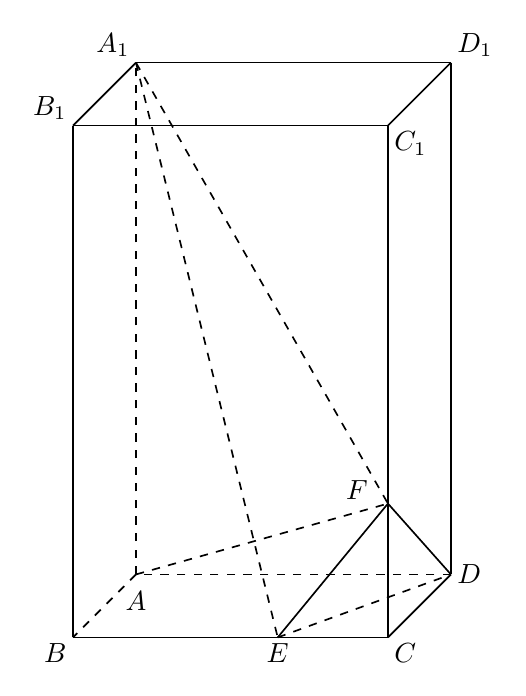
\begin{tikzpicture}[x=1cm,y=1cm,font=\normalsize,line width=.6pt]
\coordinate (B) at (0,0);
\coordinate (C) at (4,0);
\coordinate (D) at (4.8,0.8);
\coordinate (A) at (0.8,0.8);
\coordinate (E) at (2.6,0);
\coordinate (F) at (4,1.7);
\coordinate (B1) at (0,6.5);
\coordinate (C1) at (4,6.5);
\coordinate (D1) at (4.8,7.3);
\coordinate (A1) at (0.8,7.3);
% bottom face
\draw[solid] (B) -- (C);
\draw[solid] (C) -- (D);
\draw[dashed] (D) -- (A);
\draw[dashed] (A) -- (B);
% top face
\draw[solid] (B1) -- (C1);
\draw[solid] (C1) -- (D1);
\draw[solid] (D1) -- (A1);
\draw[solid] (A1) -- (B1);
% vertical edges
\draw[solid] (B) -- (B1);
\draw[solid] (C) -- (C1);
\draw[solid] (D) -- (D1);
\draw[dashed] (A) -- (A1);
% interior segments visible in original
\draw[dashed] (A1) -- (E);
\draw[dashed] (A1) -- (F);
\draw[dashed] (A) -- (F);
\draw[solid] (F) -- (E);
\draw[solid] (F) -- (D);
\draw[dashed] (E) -- (D);
\node[below left,inner sep=2pt] at (B) {$B$};
\node[below,inner sep=2pt,yshift=-4pt] at (A) {$A$};
\node[below,inner sep=2pt] at (E) {$E$};
\node[below right,inner sep=2pt] at (C) {$C$};
\node[right,inner sep=2pt] at (D) {$D$};
\node[above left,inner sep=2pt,xshift=-5pt,yshift=-1pt] at (F) {$F$};
\node[above left,inner sep=2pt] at (B1) {$B_{1}$};
\node[above left,inner sep=2pt] at (A1) {$A_{1}$};
\node[below right,inner sep=2pt] at (C1) {$C_{1}$};
\node[above right,inner sep=2pt] at (D1) {$D_{1}$};
\end{tikzpicture}
